\documentclass[1p]{elsarticle_modified}
%\bibliographystyle{elsarticle-num}

%\usepackage[colorlinks]{hyperref}
%\usepackage{abbrmath_seonhwa} %\Abb, \Ascr, \Acal ,\Abf, \Afrak
\usepackage{amsfonts}
\usepackage{amssymb}
\usepackage{amsmath}
\usepackage{amsthm}
\usepackage{scalefnt}
\usepackage{amsbsy}
\usepackage{kotex}
\usepackage{caption}
\usepackage{subfig}
\usepackage{color}
\usepackage{graphicx}
\usepackage{xcolor} %% white, black, red, green, blue, cyan, magenta, yellow
\usepackage{float}
\usepackage{setspace}
\usepackage{hyperref}

\usepackage{tikz}
\usetikzlibrary{arrows}

\usepackage{multirow}
\usepackage{array} % fixed length table
\usepackage{hhline}

%%%%%%%%%%%%%%%%%%%%%
\makeatletter
\renewcommand*\env@matrix[1][\arraystretch]{%
	\edef\arraystretch{#1}%
	\hskip -\arraycolsep
	\let\@ifnextchar\new@ifnextchar
	\array{*\c@MaxMatrixCols c}}
\makeatother %https://tex.stackexchange.com/questions/14071/how-can-i-increase-the-line-spacing-in-a-matrix
%%%%%%%%%%%%%%%

\usepackage[normalem]{ulem}

\newcommand{\msout}[1]{\ifmmode\text{\sout{\ensuremath{#1}}}\else\sout{#1}\fi}
%SOURCE: \msout is \stkout macro in https://tex.stackexchange.com/questions/20609/strikeout-in-math-mode

\newcommand{\cancel}[1]{
	\ifmmode
	{\color{red}\msout{#1}}
	\else
	{\color{red}\sout{#1}}
	\fi
}

\newcommand{\add}[1]{
	{\color{blue}\uwave{#1}}
}

\newcommand{\replace}[2]{
	\ifmmode
	{\color{red}\msout{#1}}{\color{blue}\uwave{#2}}
	\else
	{\color{red}\sout{#1}}{\color{blue}\uwave{#2}}
	\fi
}

\newcommand{\Sol}{\mathcal{S}} %segment
\newcommand{\D}{D} %diagram
\newcommand{\A}{\mathcal{A}} %arc


%%%%%%%%%%%%%%%%%%%%%%%%%%%%%5 test

\def\sl{\operatorname{\textup{SL}}(2,\Cbb)}
\def\psl{\operatorname{\textup{PSL}}(2,\Cbb)}
\def\quan{\mkern 1mu \triangleright \mkern 1mu}

\theoremstyle{definition}
\newtheorem{thm}{Theorem}[section]
\newtheorem{prop}[thm]{Proposition}
\newtheorem{lem}[thm]{Lemma}
\newtheorem{ques}[thm]{Question}
\newtheorem{cor}[thm]{Corollary}
\newtheorem{defn}[thm]{Definition}
\newtheorem{exam}[thm]{Example}
\newtheorem{rmk}[thm]{Remark}
\newtheorem{alg}[thm]{Algorithm}

\newcommand{\I}{\sqrt{-1}}
\begin{document}

%\begin{frontmatter}
%
%\title{Boundary parabolic representations of knots up to 8 crossings}
%
%%% Group authors per affiliation:
%\author{Yunhi Cho} 
%\address{Department of Mathematics, University of Seoul, Seoul, Korea}
%\ead{yhcho@uos.ac.kr}
%
%
%\author{Seonhwa Kim} %\fnref{s_kim}}
%\address{Center for Geometry and Physics, Institute for Basic Science, Pohang, 37673, Korea}
%\ead{ryeona17@ibs.re.kr}
%
%\author{Hyuk Kim}
%\address{Department of Mathematical Sciences, Seoul National University, Seoul 08826, Korea}
%\ead{hyukkim@snu.ac.kr}
%
%\author{Seokbeom Yoon}
%\address{Department of Mathematical Sciences, Seoul National University, Seoul, 08826,  Korea}
%\ead{sbyoon15@snu.ac.kr}
%
%\begin{abstract}
%We find all boundary parabolic representation of knots up to 8 crossings.
%
%\end{abstract}
%\begin{keyword}
%    \MSC[2010] 57M25 
%\end{keyword}
%
%\end{frontmatter}

%\linenumbers
%\tableofcontents
%
\newcommand\colored[1]{\textcolor{white}{\rule[-0.35ex]{0.8em}{1.4ex}}\kern-0.8em\color{red} #1}%
%\newcommand\colored[1]{\textcolor{white}{ #1}\kern-2.17ex	\textcolor{white}{ #1}\kern-1.81ex	\textcolor{white}{ #1}\kern-2.15ex\color{red}#1	}

{\Large $\underline{12a_{0623}~(K12a_{0623})}$}

\setlength{\tabcolsep}{10pt}
\renewcommand{\arraystretch}{1.6}
\vspace{1cm}\begin{tabular}{m{100pt}>{\centering\arraybackslash}m{274pt}}
\multirow{5}{120pt}{
	\centering
	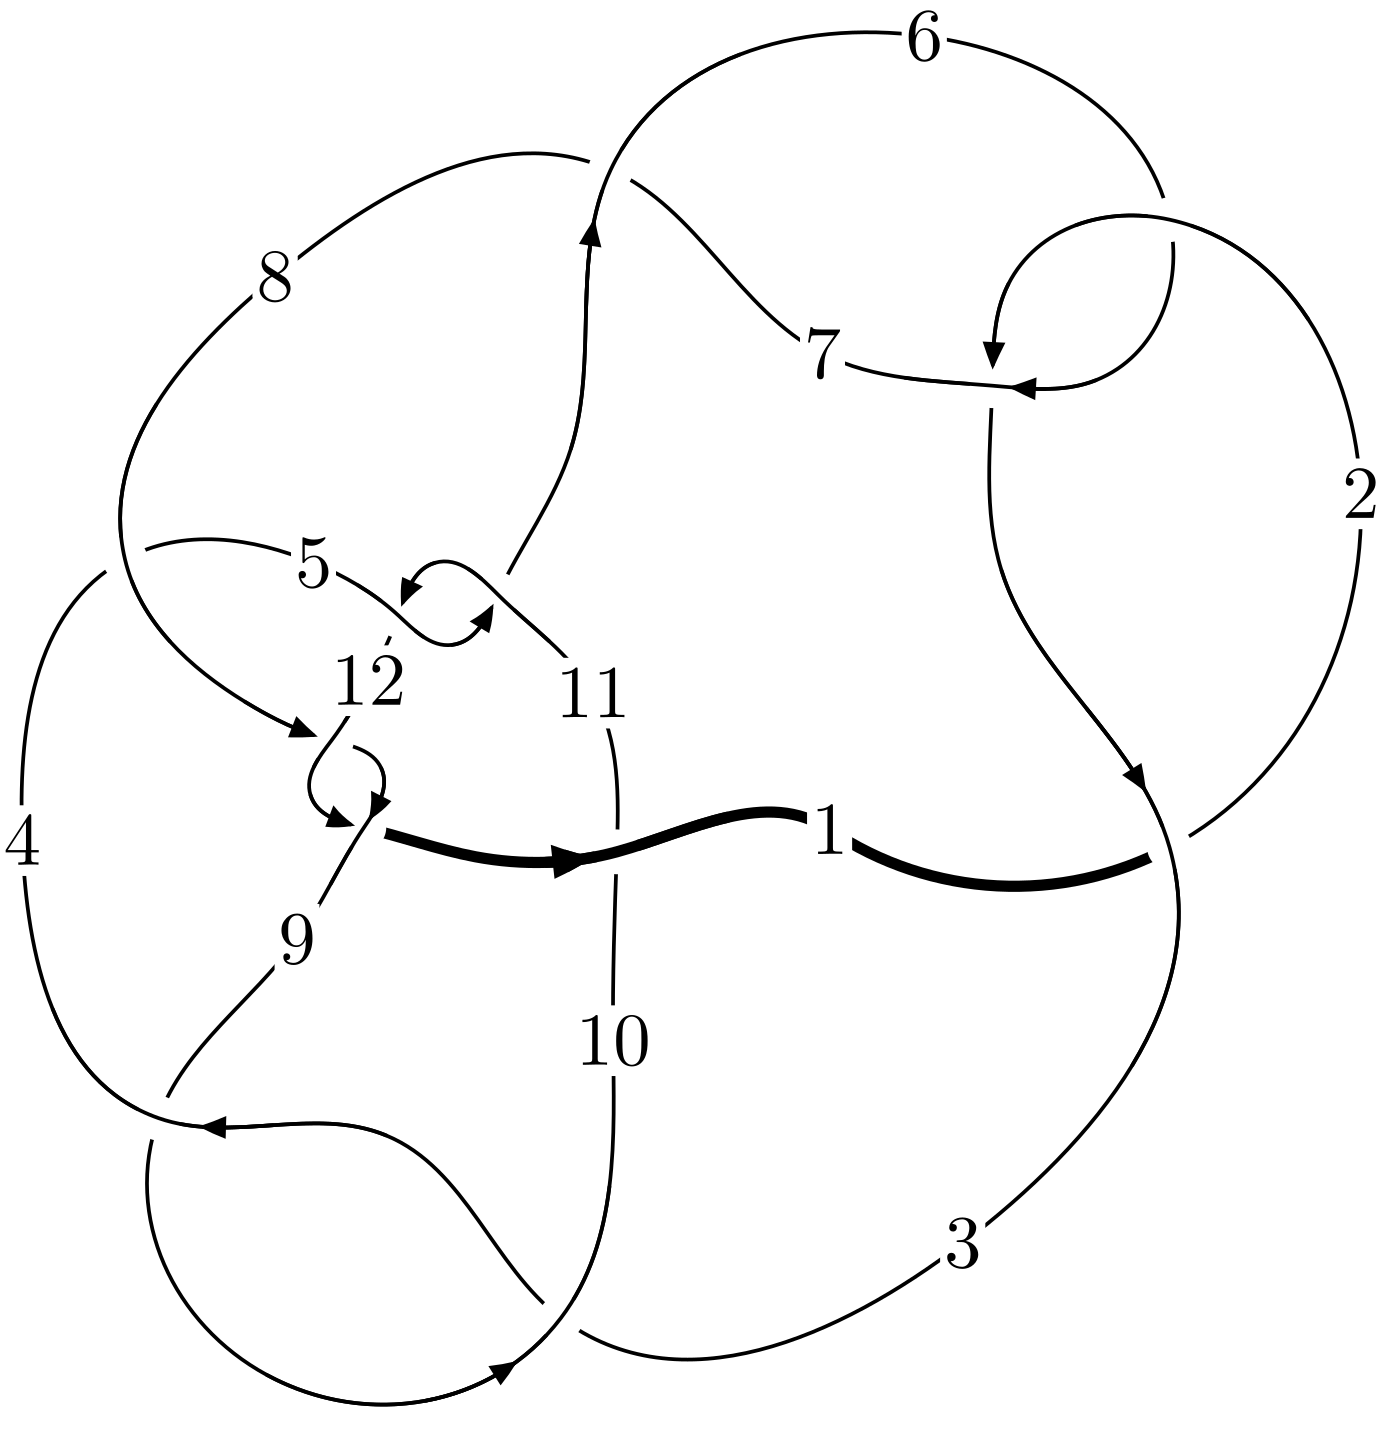
\includegraphics[width=112pt]{../../../GIT/diagram.site/Diagrams/png/1424_12a_0623.png}\\
\ \ \ A knot diagram\footnotemark}&
\allowdisplaybreaks
\textbf{Linearized knot diagam} \\
\cline{2-2}
 &
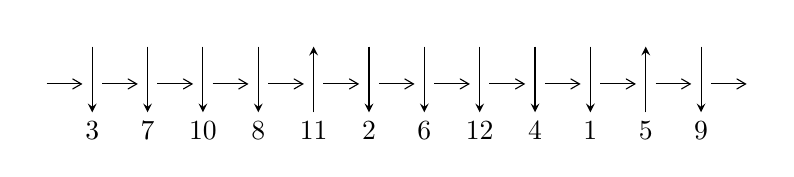
\begin{tikzpicture}[x=20pt, y=17pt]
	% nodes
	\node (C0) at (0, 0) {};
	\node (C1) at (1, 0) {};
	\node (C1U) at (1, +1) {};
	\node (C1D) at (1, -1) {3};

	\node (C2) at (2, 0) {};
	\node (C2U) at (2, +1) {};
	\node (C2D) at (2, -1) {7};

	\node (C3) at (3, 0) {};
	\node (C3U) at (3, +1) {};
	\node (C3D) at (3, -1) {10};

	\node (C4) at (4, 0) {};
	\node (C4U) at (4, +1) {};
	\node (C4D) at (4, -1) {8};

	\node (C5) at (5, 0) {};
	\node (C5U) at (5, +1) {};
	\node (C5D) at (5, -1) {11};

	\node (C6) at (6, 0) {};
	\node (C6U) at (6, +1) {};
	\node (C6D) at (6, -1) {2};

	\node (C7) at (7, 0) {};
	\node (C7U) at (7, +1) {};
	\node (C7D) at (7, -1) {6};

	\node (C8) at (8, 0) {};
	\node (C8U) at (8, +1) {};
	\node (C8D) at (8, -1) {12};

	\node (C9) at (9, 0) {};
	\node (C9U) at (9, +1) {};
	\node (C9D) at (9, -1) {4};

	\node (C10) at (10, 0) {};
	\node (C10U) at (10, +1) {};
	\node (C10D) at (10, -1) {1};

	\node (C11) at (11, 0) {};
	\node (C11U) at (11, +1) {};
	\node (C11D) at (11, -1) {5};

	\node (C12) at (12, 0) {};
	\node (C12U) at (12, +1) {};
	\node (C12D) at (12, -1) {9};
	\node (C13) at (13, 0) {};

	% arrows
	\draw[->,>={angle 60}]
	(C0) edge (C1) (C1) edge (C2) (C2) edge (C3) (C3) edge (C4) (C4) edge (C5) (C5) edge (C6) (C6) edge (C7) (C7) edge (C8) (C8) edge (C9) (C9) edge (C10) (C10) edge (C11) (C11) edge (C12) (C12) edge (C13) ;	\draw[->,>=stealth]
	(C1U) edge (C1D) (C2U) edge (C2D) (C3U) edge (C3D) (C4U) edge (C4D) (C5D) edge (C5U) (C6U) edge (C6D) (C7U) edge (C7D) (C8U) edge (C8D) (C9U) edge (C9D) (C10U) edge (C10D) (C11D) edge (C11U) (C12U) edge (C12D) ;
	\end{tikzpicture} \\
\hhline{~~} \\& 
\textbf{Solving Sequence} \\ \cline{2-2} 
 &
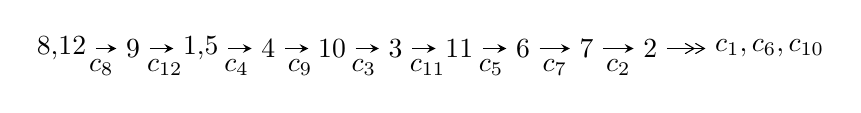
\begin{tikzpicture}[x=23pt, y=7pt]
	% node
	\node (A0) at (-1/8, 0) {8,12};
	\node (A1) at (1, 0) {9};
	\node (A2) at (33/16, 0) {1,5};
	\node (A3) at (25/8, 0) {4};
	\node (A4) at (33/8, 0) {10};
	\node (A5) at (41/8, 0) {3};
	\node (A6) at (49/8, 0) {11};
	\node (A7) at (57/8, 0) {6};
	\node (A8) at (65/8, 0) {7};
	\node (A9) at (73/8, 0) {2};
	\node (C1) at (1/2, -1) {$c_{8}$};
	\node (C2) at (3/2, -1) {$c_{12}$};
	\node (C3) at (21/8, -1) {$c_{4}$};
	\node (C4) at (29/8, -1) {$c_{9}$};
	\node (C5) at (37/8, -1) {$c_{3}$};
	\node (C6) at (45/8, -1) {$c_{11}$};
	\node (C7) at (53/8, -1) {$c_{5}$};
	\node (C8) at (61/8, -1) {$c_{7}$};
	\node (C9) at (69/8, -1) {$c_{2}$};
	\node (A10) at (11, 0) {$c_{1},c_{6},c_{10}$};

	% edge
	\draw[->,>=stealth]	
	(A0) edge (A1) (A1) edge (A2) (A2) edge (A3) (A3) edge (A4) (A4) edge (A5) (A5) edge (A6) (A6) edge (A7) (A7) edge (A8) (A8) edge (A9) ;
	\draw[->>,>={angle 60}]	
	(A9) edge (A10);
\end{tikzpicture} \\ 

\end{tabular} \\

\footnotetext{
The image of knot diagram is generated by the software ``\textbf{Draw programme}" developed by Andrew Bartholomew(\url{http://www.layer8.co.uk/maths/draw/index.htm\#Running-draw}), where we modified some parts for our purpose(\url{https://github.com/CATsTAILs/LinksPainter}).
}\phantom \\ \newline 
\centering \textbf{Ideals for irreducible components\footnotemark of $X_{\text{par}}$} 
 
\begin{align*}
I^u_{1}&=\langle 
-97455286 u^{69}-687147084 u^{68}+\cdots+1146617856 b-4289778370546,\\
\phantom{I^u_{1}}&\phantom{= \langle  }-2616564386981 u^{69}-14513594810490 u^{68}+\cdots+83529964191744 a-11174734769596142,\\
\phantom{I^u_{1}}&\phantom{= \langle  }u^{70}+8 u^{69}+\cdots+286521 u+48566\rangle \\
I^u_{2}&=\langle 
a^2+b,\;a^3+a+1,\;u-1\rangle \\
I^u_{3}&=\langle 
a^6 b^3+3 a^4 b^3+\cdots-2 a+1,\;u-1\rangle \\
\\
I^v_{1}&=\langle 
a,\;b^9+3 b^7- b^6+3 b^5-2 b^4+3 b^3- b^2+2 b-1,\;v-1\rangle \\
\end{align*}
\raggedright * 3 irreducible components of $\dim_{\mathbb{C}}=0$, with total 82 representations.\\
\raggedright * 1 irreducible components of $\dim_{\mathbb{C}}=1$ \\
\footnotetext{All coefficients of polynomials are rational numbers. But the coefficients are sometimes approximated in decimal forms when there is not enough margin.}
\newpage
\renewcommand{\arraystretch}{1}
\centering \section*{I. $I^u_{1}= \langle -9.75\times10^{7} u^{69}-6.87\times10^{8} u^{68}+\cdots+1.15\times10^{9} b-4.29\times10^{12},\;-2.62\times10^{12} u^{69}-1.45\times10^{13} u^{68}+\cdots+8.35\times10^{13} a-1.12\times10^{16},\;u^{70}+8 u^{69}+\cdots+286521 u+48566 \rangle$}
\flushleft \textbf{(i) Arc colorings}\\
\begin{tabular}{m{7pt} m{180pt} m{7pt} m{180pt} }
\flushright $a_{8}=$&$\begin{pmatrix}1\\0\end{pmatrix}$ \\
\flushright $a_{12}=$&$\begin{pmatrix}0\\u\end{pmatrix}$ \\
\flushright $a_{9}=$&$\begin{pmatrix}1\\u^2\end{pmatrix}$ \\
\flushright $a_{1}=$&$\begin{pmatrix}- u\\- u^3+u\end{pmatrix}$ \\
\flushright $a_{5}=$&$\begin{pmatrix}0.0313249 u^{69}+0.173753 u^{68}+\cdots+1396.40 u+133.781\\0.0849937 u^{69}+0.599282 u^{68}+\cdots+18949.7 u+3741.25\end{pmatrix}$ \\
\flushright $a_{4}=$&$\begin{pmatrix}0.116319 u^{69}+0.773035 u^{68}+\cdots+20346.1 u+3875.03\\0.0849937 u^{69}+0.599282 u^{68}+\cdots+18949.7 u+3741.25\end{pmatrix}$ \\
\flushright $a_{10}=$&$\begin{pmatrix}0.00502741 u^{69}+0.0354161 u^{68}+\cdots+1224.91 u+250.562\\0.00488338 u^{69}+0.0343100 u^{68}+\cdots+1186.75 u+242.634\end{pmatrix}$ \\
\flushright $a_{3}=$&$\begin{pmatrix}0.195712 u^{69}+1.34410 u^{68}+\cdots+39810.9 u+7746.66\\0.0226364 u^{69}+0.194253 u^{68}+\cdots+9789.24 u+2087.61\end{pmatrix}$ \\
\flushright $a_{11}=$&$\begin{pmatrix}-0.000357427 u^{69}-0.00242242 u^{68}+\cdots-69.0145 u-13.3644\\0.00530723 u^{69}+0.0369747 u^{68}+\cdots+1240.78 u+252.067\end{pmatrix}$ \\
\flushright $a_{6}=$&$\begin{pmatrix}-0.178615 u^{69}-1.22581 u^{68}+\cdots-36017.6 u-6978.08\\0.0152291 u^{69}+0.0703555 u^{68}+\cdots-1191.09 u-359.181\end{pmatrix}$ \\
\flushright $a_{7}=$&$\begin{pmatrix}0.0167391 u^{69}+0.103977 u^{68}+\cdots+1900.39 u+320.006\\0.0149456 u^{69}+0.106887 u^{68}+\cdots+3365.62 u+648.931\end{pmatrix}$ \\
\flushright $a_{2}=$&$\begin{pmatrix}0.0165738 u^{69}+0.102484 u^{68}+\cdots+1975.39 u+350.122\\0.0170226 u^{69}+0.116505 u^{68}+\cdots+3345.21 u+649.216\end{pmatrix}$\\&\end{tabular}
\flushleft \textbf{(ii) Obstruction class $= -1$}\\~\\
\flushleft \textbf{(iii) Cusp Shapes $= \frac{836940515}{5159780352} u^{69}+\frac{588646361}{573308928} u^{68}+\cdots+\frac{107767045126535}{5159780352} u+\frac{9383241457921}{2579890176}$}\\~\\
\newpage\renewcommand{\arraystretch}{1}
\flushleft \textbf{(iv) u-Polynomials at the component}\newline \\
\begin{tabular}{m{50pt}|m{274pt}}
Crossings & \hspace{64pt}u-Polynomials at each crossing \\
\hline $$\begin{aligned}c_{1},c_{7}\end{aligned}$$&$\begin{aligned}
&u^{70}+20 u^{69}+\cdots-1331 u+3844
\end{aligned}$\\
\hline $$\begin{aligned}c_{2},c_{6}\end{aligned}$$&$\begin{aligned}
&u^{70}+4 u^{69}+\cdots+163 u+62
\end{aligned}$\\
\hline $$\begin{aligned}c_{3},c_{9}\end{aligned}$$&$\begin{aligned}
&27(27 u^{70}+27 u^{69}+\cdots-6 u+1)
\end{aligned}$\\
\hline $$\begin{aligned}c_{4}\end{aligned}$$&$\begin{aligned}
&64(64 u^{70}-128 u^{69}+\cdots-118314 u+15039)
\end{aligned}$\\
\hline $$\begin{aligned}c_{5},c_{11}\end{aligned}$$&$\begin{aligned}
&27(27 u^{70}+27 u^{69}+\cdots+8 u+1)
\end{aligned}$\\
\hline $$\begin{aligned}c_{8},c_{12}\end{aligned}$$&$\begin{aligned}
&u^{70}-8 u^{69}+\cdots-286521 u+48566
\end{aligned}$\\
\hline $$\begin{aligned}c_{10}\end{aligned}$$&$\begin{aligned}
&64(64 u^{70}+96 u^{68}+\cdots+356292 u+635013)
\end{aligned}$\\
\hline
\end{tabular}\\~\\
\newpage\renewcommand{\arraystretch}{1}
\flushleft \textbf{(v) Riley Polynomials at the component}\newline \\
\begin{tabular}{m{50pt}|m{274pt}}
Crossings & \hspace{64pt}Riley Polynomials at each crossing \\
\hline $$\begin{aligned}c_{1},c_{7}\end{aligned}$$&$\begin{aligned}
&y^{70}+60 y^{69}+\cdots+419446271 y+14776336
\end{aligned}$\\
\hline $$\begin{aligned}c_{2},c_{6}\end{aligned}$$&$\begin{aligned}
&y^{70}-20 y^{69}+\cdots+1331 y+3844
\end{aligned}$\\
\hline $$\begin{aligned}c_{3},c_{9}\end{aligned}$$&$\begin{aligned}
&729(729 y^{70}+34263 y^{69}+\cdots+36 y+1)
\end{aligned}$\\
\hline $$\begin{aligned}c_{4}\end{aligned}$$&$\begin{aligned}
&4096(4096 y^{70}+28672 y^{69}+\cdots+4.67293\times10^{9} y+2.26172\times10^{8})
\end{aligned}$\\
\hline $$\begin{aligned}c_{5},c_{11}\end{aligned}$$&$\begin{aligned}
&729(729 y^{70}+31347 y^{69}+\cdots+36 y+1)
\end{aligned}$\\
\hline $$\begin{aligned}c_{8},c_{12}\end{aligned}$$&$\begin{aligned}
&y^{70}-48 y^{69}+\cdots-3572288981 y+2358656356
\end{aligned}$\\
\hline $$\begin{aligned}c_{10}\end{aligned}$$&$\begin{aligned}
&4096\\
&\cdot(4096 y^{70}+12288 y^{69}+\cdots+402241554234 y+403241510169)
\end{aligned}$\\
\hline
\end{tabular}\\~\\
\newpage\flushleft \textbf{(vi) Complex Volumes and Cusp Shapes}
$$\begin{array}{c|c|c}  
\text{Solutions to }I^u_{1}& \I (\text{vol} + \sqrt{-1}CS) & \text{Cusp shape}\\
 \hline 
\begin{aligned}
u &= \phantom{-}0.893258 + 0.388589 I \\
a &= -0.552997 - 0.780965 I \\
b &= \phantom{-}0.717124 - 0.518987 I\end{aligned}
 & -0.32512 - 1.94198 I & -8.00000 + 0. I\phantom{ +0.000000I} \\ \hline\begin{aligned}
u &= \phantom{-}0.893258 - 0.388589 I \\
a &= -0.552997 + 0.780965 I \\
b &= \phantom{-}0.717124 + 0.518987 I\end{aligned}
 & -0.32512 + 1.94198 I & -8.00000 + 0. I\phantom{ +0.000000I} \\ \hline\begin{aligned}
u &= \phantom{-}0.885513 + 0.566554 I \\
a &= \phantom{-}0.648570 + 0.785318 I \\
b &= -0.921742 + 0.293488 I\end{aligned}
 & -1.00008 + 3.25130 I & \phantom{-0.000000 } 0 \\ \hline\begin{aligned}
u &= \phantom{-}0.885513 - 0.566554 I \\
a &= \phantom{-}0.648570 - 0.785318 I \\
b &= -0.921742 - 0.293488 I\end{aligned}
 & -1.00008 - 3.25130 I & \phantom{-0.000000 } 0 \\ \hline\begin{aligned}
u &= -0.976800 + 0.399121 I \\
a &= \phantom{-}0.294251 + 0.362673 I \\
b &= \phantom{-}1.260270 + 0.039825 I\end{aligned}
 & -1.84431 + 1.78184 I & \phantom{-0.000000 } 0 \\ \hline\begin{aligned}
u &= -0.976800 - 0.399121 I \\
a &= \phantom{-}0.294251 - 0.362673 I \\
b &= \phantom{-}1.260270 - 0.039825 I\end{aligned}
 & -1.84431 - 1.78184 I & \phantom{-0.000000 } 0 \\ \hline\begin{aligned}
u &= -0.215479 + 0.892593 I \\
a &= -0.085570 + 1.030780 I \\
b &= -0.163375 - 1.188040 I\end{aligned}
 & \phantom{-}9.48735 - 0.61216 I & \phantom{-0.000000 }      -6
0. 10   - 1.258234 I \\ \hline\begin{aligned}
u &= -0.215479 - 0.892593 I \\
a &= -0.085570 - 1.030780 I \\
b &= -0.163375 + 1.188040 I\end{aligned}
 & \phantom{-}9.48735 + 0.61216 I & \phantom{-0.000000 -}     -6
0. 10   + 1.258234 I \\ \hline\begin{aligned}
u &= \phantom{-}1.095420 + 0.120474 I \\
a &= -0.219567 - 0.414390 I \\
b &= \phantom{-}0.221171 - 1.058020 I\end{aligned}
 & -2.53231 + 0.75873 I & \phantom{-0.000000 } 0 \\ \hline\begin{aligned}
u &= \phantom{-}1.095420 - 0.120474 I \\
a &= -0.219567 + 0.414390 I \\
b &= \phantom{-}0.221171 + 1.058020 I\end{aligned}
 & -2.53231 - 0.75873 I & \phantom{-0.000000 } 0\\
 \hline 
 \end{array}$$\newpage$$\begin{array}{c|c|c}  
\text{Solutions to }I^u_{1}& \I (\text{vol} + \sqrt{-1}CS) & \text{Cusp shape}\\
 \hline 
\begin{aligned}
u &= -0.199757 + 0.871147 I \\
a &= -0.003629 - 1.084200 I \\
b &= \phantom{-}0.234615 + 1.216000 I\end{aligned}
 & \phantom{-}8.94654 - 6.79753 I & -1.43725 + 3.99331 I \\ \hline\begin{aligned}
u &= -0.199757 - 0.871147 I \\
a &= -0.003629 + 1.084200 I \\
b &= \phantom{-}0.234615 - 1.216000 I\end{aligned}
 & \phantom{-}8.94654 + 6.79753 I & -1.43725 - 3.99331 I \\ \hline\begin{aligned}
u &= -0.047582 + 1.166560 I \\
a &= \phantom{-}1.014120 - 0.495065 I \\
b &= -0.731641 + 0.839705 I\end{aligned}
 & \phantom{-}5.86206 + 12.07860 I & \phantom{-0.000000 } 0 \\ \hline\begin{aligned}
u &= -0.047582 - 1.166560 I \\
a &= \phantom{-}1.014120 + 0.495065 I \\
b &= -0.731641 - 0.839705 I\end{aligned}
 & \phantom{-}5.86206 - 12.07860 I & \phantom{-0.000000 } 0 \\ \hline\begin{aligned}
u &= \phantom{-}0.351855 + 0.750985 I \\
a &= \phantom{-}1.106910 + 0.809645 I \\
b &= -0.921640 - 0.132570 I\end{aligned}
 & -4.19660 - 2.54473 I & -15.7326 + 4.0183 I \\ \hline\begin{aligned}
u &= \phantom{-}0.351855 - 0.750985 I \\
a &= \phantom{-}1.106910 - 0.809645 I \\
b &= -0.921640 + 0.132570 I\end{aligned}
 & -4.19660 + 2.54473 I & -15.7326 - 4.0183 I \\ \hline\begin{aligned}
u &= -0.082928 + 1.177070 I \\
a &= -0.924676 + 0.521308 I \\
b &= \phantom{-}0.643758 - 0.842940 I\end{aligned}
 & \phantom{-}6.91710 + 5.79367 I & \phantom{-0.000000 } 0 \\ \hline\begin{aligned}
u &= -0.082928 - 1.177070 I \\
a &= -0.924676 - 0.521308 I \\
b &= \phantom{-}0.643758 + 0.842940 I\end{aligned}
 & \phantom{-}6.91710 - 5.79367 I & \phantom{-0.000000 } 0 \\ \hline\begin{aligned}
u &= -1.086210 + 0.503549 I \\
a &= -0.574505 - 0.269617 I \\
b &= -0.770399 + 0.355339 I\end{aligned}
 & \phantom{-}1.74908 + 3.93961 I & \phantom{-0.000000 } 0 \\ \hline\begin{aligned}
u &= -1.086210 - 0.503549 I \\
a &= -0.574505 + 0.269617 I \\
b &= -0.770399 - 0.355339 I\end{aligned}
 & \phantom{-}1.74908 - 3.93961 I & \phantom{-0.000000 } 0\\
 \hline 
 \end{array}$$\newpage$$\begin{array}{c|c|c}  
\text{Solutions to }I^u_{1}& \I (\text{vol} + \sqrt{-1}CS) & \text{Cusp shape}\\
 \hline 
\begin{aligned}
u &= -1.134340 + 0.450358 I \\
a &= \phantom{-}0.649347 + 0.472023 I \\
b &= \phantom{-}0.936842 - 0.641523 I\end{aligned}
 & -0.87100 + 7.24185 I & \phantom{-0.000000 } 0 \\ \hline\begin{aligned}
u &= -1.134340 - 0.450358 I \\
a &= \phantom{-}0.649347 - 0.472023 I \\
b &= \phantom{-}0.936842 + 0.641523 I\end{aligned}
 & -0.87100 - 7.24185 I & \phantom{-0.000000 } 0 \\ \hline\begin{aligned}
u &= \phantom{-}0.163320 + 0.751919 I \\
a &= \phantom{-}1.28394 + 0.96111 I \\
b &= -1.070540 - 0.431024 I\end{aligned}
 & \phantom{-}1.13016 - 7.73289 I & -7.91932 + 7.41023 I \\ \hline\begin{aligned}
u &= \phantom{-}0.163320 - 0.751919 I \\
a &= \phantom{-}1.28394 - 0.96111 I \\
b &= -1.070540 + 0.431024 I\end{aligned}
 & \phantom{-}1.13016 + 7.73289 I & -7.91932 - 7.41023 I \\ \hline\begin{aligned}
u &= -0.312077 + 0.680537 I \\
a &= -0.354528 - 0.535888 I \\
b &= \phantom{-}0.398075 + 0.893488 I\end{aligned}
 & \phantom{-}1.65608 - 2.83282 I & -3.61063 + 4.56409 I \\ \hline\begin{aligned}
u &= -0.312077 - 0.680537 I \\
a &= -0.354528 + 0.535888 I \\
b &= \phantom{-}0.398075 - 0.893488 I\end{aligned}
 & \phantom{-}1.65608 + 2.83282 I & -3.61063 - 4.56409 I \\ \hline\begin{aligned}
u &= -1.267440 + 0.034085 I \\
a &= \phantom{-}0.013948 + 0.738018 I \\
b &= \phantom{-}0.27952 - 2.11838 I\end{aligned}
 & \phantom{-}0.08596 + 3.02639 I & \phantom{-0.000000 } 0 \\ \hline\begin{aligned}
u &= -1.267440 - 0.034085 I \\
a &= \phantom{-}0.013948 - 0.738018 I \\
b &= \phantom{-}0.27952 + 2.11838 I\end{aligned}
 & \phantom{-}0.08596 - 3.02639 I & \phantom{-0.000000 } 0 \\ \hline\begin{aligned}
u &= \phantom{-}0.145804 + 0.711603 I \\
a &= -1.23500 - 0.98762 I \\
b &= \phantom{-}0.980444 + 0.490899 I\end{aligned}
 & \phantom{-}1.85042 - 2.01318 I & -6.24038 + 2.74940 I \\ \hline\begin{aligned}
u &= \phantom{-}0.145804 - 0.711603 I \\
a &= -1.23500 + 0.98762 I \\
b &= \phantom{-}0.980444 - 0.490899 I\end{aligned}
 & \phantom{-}1.85042 + 2.01318 I & -6.24038 - 2.74940 I\\
 \hline 
 \end{array}$$\newpage$$\begin{array}{c|c|c}  
\text{Solutions to }I^u_{1}& \I (\text{vol} + \sqrt{-1}CS) & \text{Cusp shape}\\
 \hline 
\begin{aligned}
u &= -1.175260 + 0.493835 I \\
a &= -0.883929 - 0.354754 I \\
b &= -0.629453 + 0.782986 I\end{aligned}
 & \phantom{-}6.52426 + 5.60100 I & \phantom{-0.000000 } 0 \\ \hline\begin{aligned}
u &= -1.175260 - 0.493835 I \\
a &= -0.883929 + 0.354754 I \\
b &= -0.629453 - 0.782986 I\end{aligned}
 & \phantom{-}6.52426 - 5.60100 I & \phantom{-0.000000 } 0 \\ \hline\begin{aligned}
u &= -1.179980 + 0.484001 I \\
a &= \phantom{-}0.901317 + 0.412933 I \\
b &= \phantom{-}0.676364 - 0.838798 I\end{aligned}
 & \phantom{-}5.92952 + 11.69500 I & \phantom{-0.000000 } 0 \\ \hline\begin{aligned}
u &= -1.179980 - 0.484001 I \\
a &= \phantom{-}0.901317 - 0.412933 I \\
b &= \phantom{-}0.676364 + 0.838798 I\end{aligned}
 & \phantom{-}5.92952 - 11.69500 I & \phantom{-0.000000 } 0 \\ \hline\begin{aligned}
u &= -0.638279 + 1.121600 I \\
a &= -0.342951 + 0.347949 I \\
b &= \phantom{-}0.012985 - 0.537783 I\end{aligned}
 & \phantom{-}3.62133 + 1.34127 I & \phantom{-0.000000 } 0 \\ \hline\begin{aligned}
u &= -0.638279 - 1.121600 I \\
a &= -0.342951 - 0.347949 I \\
b &= \phantom{-}0.012985 + 0.537783 I\end{aligned}
 & \phantom{-}3.62133 - 1.34127 I & \phantom{-0.000000 } 0 \\ \hline\begin{aligned}
u &= -1.285690 + 0.354856 I \\
a &= \phantom{-}0.220687 + 1.116770 I \\
b &= \phantom{-}1.27101 - 0.92407 I\end{aligned}
 & -2.48686 + 5.88009 I & \phantom{-0.000000 } 0 \\ \hline\begin{aligned}
u &= -1.285690 - 0.354856 I \\
a &= \phantom{-}0.220687 - 1.116770 I \\
b &= \phantom{-}1.27101 + 0.92407 I\end{aligned}
 & -2.48686 - 5.88009 I & \phantom{-0.000000 } 0 \\ \hline\begin{aligned}
u &= -0.651619 + 0.094400 I \\
a &= -0.051734 + 0.517565 I \\
b &= \phantom{-}0.39702 + 1.63749 I\end{aligned}
 & \phantom{-}2.36312 - 2.67944 I & \phantom{-}0.83747 + 1.99355 I \\ \hline\begin{aligned}
u &= -0.651619 - 0.094400 I \\
a &= -0.051734 - 0.517565 I \\
b &= \phantom{-}0.39702 - 1.63749 I\end{aligned}
 & \phantom{-}2.36312 + 2.67944 I & \phantom{-}0.83747 - 1.99355 I\\
 \hline 
 \end{array}$$\newpage$$\begin{array}{c|c|c}  
\text{Solutions to }I^u_{1}& \I (\text{vol} + \sqrt{-1}CS) & \text{Cusp shape}\\
 \hline 
\begin{aligned}
u &= -1.293020 + 0.364510 I \\
a &= -0.199843 - 1.172110 I \\
b &= -1.29020 + 0.89246 I\end{aligned}
 & -3.28892 + 11.74160 I & \phantom{-0.000000 } 0 \\ \hline\begin{aligned}
u &= -1.293020 - 0.364510 I \\
a &= -0.199843 + 1.172110 I \\
b &= -1.29020 - 0.89246 I\end{aligned}
 & -3.28892 - 11.74160 I & \phantom{-0.000000 } 0 \\ \hline\begin{aligned}
u &= -1.327690 + 0.292888 I \\
a &= \phantom{-}0.061634 + 0.954982 I \\
b &= \phantom{-}1.05038 - 0.97956 I\end{aligned}
 & -5.50505 + 3.76007 I & \phantom{-0.000000 } 0 \\ \hline\begin{aligned}
u &= -1.327690 - 0.292888 I \\
a &= \phantom{-}0.061634 - 0.954982 I \\
b &= \phantom{-}1.05038 + 0.97956 I\end{aligned}
 & -5.50505 - 3.76007 I & \phantom{-0.000000 } 0 \\ \hline\begin{aligned}
u &= -0.959797 + 0.964946 I \\
a &= -0.363592 + 0.229548 I \\
b &= -0.107376 - 0.290881 I\end{aligned}
 & \phantom{-}3.60962 + 1.37846 I & \phantom{-0.000000 } 0 \\ \hline\begin{aligned}
u &= -0.959797 - 0.964946 I \\
a &= -0.363592 - 0.229548 I \\
b &= -0.107376 + 0.290881 I\end{aligned}
 & \phantom{-}3.60962 - 1.37846 I & \phantom{-0.000000 } 0 \\ \hline\begin{aligned}
u &= -1.329050 + 0.345273 I \\
a &= -0.045275 - 1.092050 I \\
b &= -1.15508 + 0.82929 I\end{aligned}
 & -9.22838 + 6.41936 I & \phantom{-0.000000 } 0 \\ \hline\begin{aligned}
u &= -1.329050 - 0.345273 I \\
a &= -0.045275 + 1.092050 I \\
b &= -1.15508 - 0.82929 I\end{aligned}
 & -9.22838 - 6.41936 I & \phantom{-0.000000 } 0 \\ \hline\begin{aligned}
u &= \phantom{-}1.384970 + 0.062679 I \\
a &= -0.0888781 + 0.0984540 I \\
b &= \phantom{-}0.004223 - 1.355380 I\end{aligned}
 & \phantom{-}3.40691 + 3.12614 I & \phantom{-0.000000 } 0 \\ \hline\begin{aligned}
u &= \phantom{-}1.384970 - 0.062679 I \\
a &= -0.0888781 - 0.0984540 I \\
b &= \phantom{-}0.004223 + 1.355380 I\end{aligned}
 & \phantom{-}3.40691 - 3.12614 I & \phantom{-0.000000 } 0\\
 \hline 
 \end{array}$$\newpage$$\begin{array}{c|c|c}  
\text{Solutions to }I^u_{1}& \I (\text{vol} + \sqrt{-1}CS) & \text{Cusp shape}\\
 \hline 
\begin{aligned}
u &= \phantom{-}0.01228 + 1.43319 I \\
a &= \phantom{-}0.765224 - 0.164117 I \\
b &= -0.600894 + 0.466851 I\end{aligned}
 & -1.44075 + 5.42106 I & \phantom{-0.000000 } 0 \\ \hline\begin{aligned}
u &= \phantom{-}0.01228 - 1.43319 I \\
a &= \phantom{-}0.765224 + 0.164117 I \\
b &= -0.600894 - 0.466851 I\end{aligned}
 & -1.44075 - 5.42106 I & \phantom{-0.000000 } 0 \\ \hline\begin{aligned}
u &= -1.40114 + 0.30543 I \\
a &= \phantom{-}0.071097 - 0.933368 I \\
b &= -0.855621 + 0.811549 I\end{aligned}
 & -8.14596 + 0.05000 I & \phantom{-0.000000 } 0 \\ \hline\begin{aligned}
u &= -1.40114 - 0.30543 I \\
a &= \phantom{-}0.071097 + 0.933368 I \\
b &= -0.855621 - 0.811549 I\end{aligned}
 & -8.14596 - 0.05000 I & \phantom{-0.000000 } 0 \\ \hline\begin{aligned}
u &= \phantom{-}1.38518 + 0.55050 I \\
a &= -0.015502 + 1.021740 I \\
b &= -1.48665 - 1.26538 I\end{aligned}
 & \phantom{-}1.3953 - 18.0795 I & \phantom{-0.000000 } 0 \\ \hline\begin{aligned}
u &= \phantom{-}1.38518 - 0.55050 I \\
a &= -0.015502 - 1.021740 I \\
b &= -1.48665 + 1.26538 I\end{aligned}
 & \phantom{-}1.3953 + 18.0795 I & \phantom{-0.000000 } 0 \\ \hline\begin{aligned}
u &= \phantom{-}1.39507 + 0.55017 I \\
a &= \phantom{-}0.027764 - 0.989036 I \\
b &= \phantom{-}1.41776 + 1.26916 I\end{aligned}
 & \phantom{-}2.33215 - 11.82430 I & \phantom{-0.000000 } 0 \\ \hline\begin{aligned}
u &= \phantom{-}1.39507 - 0.55017 I \\
a &= \phantom{-}0.027764 + 0.989036 I \\
b &= \phantom{-}1.41776 - 1.26916 I\end{aligned}
 & \phantom{-}2.33215 + 11.82430 I & \phantom{-0.000000 } 0 \\ \hline\begin{aligned}
u &= \phantom{-}1.39216 + 0.59468 I \\
a &= \phantom{-}0.093686 + 0.940274 I \\
b &= -1.39504 - 1.00978 I\end{aligned}
 & -5.80113 - 12.08780 I & \phantom{-0.000000 } 0 \\ \hline\begin{aligned}
u &= \phantom{-}1.39216 - 0.59468 I \\
a &= \phantom{-}0.093686 - 0.940274 I \\
b &= -1.39504 + 1.00978 I\end{aligned}
 & -5.80113 + 12.08780 I & \phantom{-0.000000 } 0\\
 \hline 
 \end{array}$$\newpage$$\begin{array}{c|c|c}  
\text{Solutions to }I^u_{1}& \I (\text{vol} + \sqrt{-1}CS) & \text{Cusp shape}\\
 \hline 
\begin{aligned}
u &= \phantom{-}0.273311 + 0.365651 I \\
a &= -1.17605 - 1.31593 I \\
b &= \phantom{-}0.455887 + 0.275732 I\end{aligned}
 & -0.556921 - 1.030040 I & -7.85697 + 6.36655 I \\ \hline\begin{aligned}
u &= \phantom{-}0.273311 - 0.365651 I \\
a &= -1.17605 + 1.31593 I \\
b &= \phantom{-}0.455887 - 0.275732 I\end{aligned}
 & -0.556921 + 1.030040 I & -7.85697 - 6.36655 I \\ \hline\begin{aligned}
u &= \phantom{-}1.44491 + 0.60643 I \\
a &= -0.064046 - 0.828480 I \\
b &= \phantom{-}1.16426 + 1.00461 I\end{aligned}
 & -1.97882 - 8.19603 I & \phantom{-0.000000 } 0 \\ \hline\begin{aligned}
u &= \phantom{-}1.44491 - 0.60643 I \\
a &= -0.064046 + 0.828480 I \\
b &= \phantom{-}1.16426 - 1.00461 I\end{aligned}
 & -1.97882 + 8.19603 I & \phantom{-0.000000 } 0 \\ \hline\begin{aligned}
u &= \phantom{-}1.42868 + 0.71532 I \\
a &= \phantom{-}0.208526 + 0.758552 I \\
b &= -1.108370 - 0.691160 I\end{aligned}
 & -6.08462 - 4.27997 I & \phantom{-0.000000 } 0 \\ \hline\begin{aligned}
u &= \phantom{-}1.42868 - 0.71532 I \\
a &= \phantom{-}0.208526 - 0.758552 I \\
b &= -1.108370 + 0.691160 I\end{aligned}
 & -6.08462 + 4.27997 I & \phantom{-0.000000 } 0 \\ \hline\begin{aligned}
u &= -1.61721 + 0.94908 I \\
a &= \phantom{-}0.353318 - 0.398464 I \\
b &= -0.174161 + 0.196426 I\end{aligned}
 & \phantom{-}1.64897 - 5.03310 I & \phantom{-0.000000 } 0 \\ \hline\begin{aligned}
u &= -1.61721 - 0.94908 I \\
a &= \phantom{-}0.353318 + 0.398464 I \\
b &= -0.174161 - 0.196426 I\end{aligned}
 & \phantom{-}1.64897 + 5.03310 I & \phantom{-0.000000 } 0 \\ \hline\begin{aligned}
u &= \phantom{-}1.92964 + 0.33599 I \\
a &= -0.004191 - 0.434882 I \\
b &= \phantom{-}0.260469 + 0.905894 I\end{aligned}
 & \phantom{-}3.22024 - 3.60088 I & \phantom{-0.000000 } 0 \\ \hline\begin{aligned}
u &= \phantom{-}1.92964 - 0.33599 I \\
a &= -0.004191 + 0.434882 I \\
b &= \phantom{-}0.260469 - 0.905894 I\end{aligned}
 & \phantom{-}3.22024 + 3.60088 I & \phantom{-0.000000 } 0\\
 \hline 
 \end{array}$$\newpage\newpage\renewcommand{\arraystretch}{1}
\centering \section*{II. $I^u_{2}= \langle a^2+b,\;a^3+a+1,\;u-1 \rangle$}
\flushleft \textbf{(i) Arc colorings}\\
\begin{tabular}{m{7pt} m{180pt} m{7pt} m{180pt} }
\flushright $a_{8}=$&$\begin{pmatrix}1\\0\end{pmatrix}$ \\
\flushright $a_{12}=$&$\begin{pmatrix}0\\1\end{pmatrix}$ \\
\flushright $a_{9}=$&$\begin{pmatrix}1\\1\end{pmatrix}$ \\
\flushright $a_{1}=$&$\begin{pmatrix}-1\\0\end{pmatrix}$ \\
\flushright $a_{5}=$&$\begin{pmatrix}a\\- a^2\end{pmatrix}$ \\
\flushright $a_{4}=$&$\begin{pmatrix}- a^2+a\\- a^2\end{pmatrix}$ \\
\flushright $a_{10}=$&$\begin{pmatrix}- a^2- a\\- a\end{pmatrix}$ \\
\flushright $a_{3}=$&$\begin{pmatrix}-1\\0\end{pmatrix}$ \\
\flushright $a_{11}=$&$\begin{pmatrix}- a^2\\- a\end{pmatrix}$ \\
\flushright $a_{6}=$&$\begin{pmatrix}-1\\0\end{pmatrix}$ \\
\flushright $a_{7}=$&$\begin{pmatrix}1\\0\end{pmatrix}$ \\
\flushright $a_{2}=$&$\begin{pmatrix}-1\\0\end{pmatrix}$\\&\end{tabular}
\flushleft \textbf{(ii) Obstruction class $= -1$}\\~\\
\flushleft \textbf{(iii) Cusp Shapes $= -6$}\\~\\
\newpage\renewcommand{\arraystretch}{1}
\flushleft \textbf{(iv) u-Polynomials at the component}\newline \\
\begin{tabular}{m{50pt}|m{274pt}}
Crossings & \hspace{64pt}u-Polynomials at each crossing \\
\hline $$\begin{aligned}c_{1},c_{2},c_{6}\\c_{7}\end{aligned}$$&$\begin{aligned}
&u^3
\end{aligned}$\\
\hline $$\begin{aligned}c_{3},c_{5},c_{9}\\c_{10},c_{11}\end{aligned}$$&$\begin{aligned}
&u^3+u+1
\end{aligned}$\\
\hline $$\begin{aligned}c_{4}\end{aligned}$$&$\begin{aligned}
&u^3+2 u^2+u-1
\end{aligned}$\\
\hline $$\begin{aligned}c_{8},c_{12}\end{aligned}$$&$\begin{aligned}
&(u+1)^3
\end{aligned}$\\
\hline
\end{tabular}\\~\\
\newpage\renewcommand{\arraystretch}{1}
\flushleft \textbf{(v) Riley Polynomials at the component}\newline \\
\begin{tabular}{m{50pt}|m{274pt}}
Crossings & \hspace{64pt}Riley Polynomials at each crossing \\
\hline $$\begin{aligned}c_{1},c_{2},c_{6}\\c_{7}\end{aligned}$$&$\begin{aligned}
&y^3
\end{aligned}$\\
\hline $$\begin{aligned}c_{3},c_{5},c_{9}\\c_{10},c_{11}\end{aligned}$$&$\begin{aligned}
&y^3+2 y^2+y-1
\end{aligned}$\\
\hline $$\begin{aligned}c_{4}\end{aligned}$$&$\begin{aligned}
&y^3-2 y^2+5 y-1
\end{aligned}$\\
\hline $$\begin{aligned}c_{8},c_{12}\end{aligned}$$&$\begin{aligned}
&(y-1)^3
\end{aligned}$\\
\hline
\end{tabular}\\~\\
\newpage\flushleft \textbf{(vi) Complex Volumes and Cusp Shapes}
$$\begin{array}{c|c|c}  
\text{Solutions to }I^u_{2}& \I (\text{vol} + \sqrt{-1}CS) & \text{Cusp shape}\\
 \hline 
\begin{aligned}
u &= \phantom{-}1.00000\phantom{ +0.000000I} \\
a &= \phantom{-}0.341164 + 1.161540 I \\
b &= \phantom{-}1.23279 - 0.79255 I\end{aligned}
 & -1.64493\phantom{ +0.000000I} & -6.00000\phantom{ +0.000000I} \\ \hline\begin{aligned}
u &= \phantom{-}1.00000\phantom{ +0.000000I} \\
a &= \phantom{-}0.341164 - 1.161540 I \\
b &= \phantom{-}1.23279 + 0.79255 I\end{aligned}
 & -1.64493\phantom{ +0.000000I} & -6.00000\phantom{ +0.000000I} \\ \hline\begin{aligned}
u &= \phantom{-}1.00000\phantom{ +0.000000I} \\
a &= -0.682328\phantom{ +0.000000I} \\
b &= -0.465571\phantom{ +0.000000I}\end{aligned}
 & -1.64493\phantom{ +0.000000I} & -6.00000\phantom{ +0.000000I}\\
 \hline 
 \end{array}$$\newpage\newpage\renewcommand{\arraystretch}{1}
\centering \section*{III. $I^u_{3}= \langle a^6 b^3+3 a^4 b^3+\cdots-2 a+1,\;u-1 \rangle$}
\flushleft \textbf{(i) Arc colorings}\\
\begin{tabular}{m{7pt} m{180pt} m{7pt} m{180pt} }
\flushright $a_{8}=$&$\begin{pmatrix}1\\0\end{pmatrix}$ \\
\flushright $a_{12}=$&$\begin{pmatrix}0\\1\end{pmatrix}$ \\
\flushright $a_{9}=$&$\begin{pmatrix}1\\1\end{pmatrix}$ \\
\flushright $a_{1}=$&$\begin{pmatrix}-1\\0\end{pmatrix}$ \\
\flushright $a_{5}=$&$\begin{pmatrix}a\\b\end{pmatrix}$ \\
\flushright $a_{4}=$&$\begin{pmatrix}b+a\\b\end{pmatrix}$ \\
\flushright $a_{10}=$&$\begin{pmatrix}- b a- a^2+1\\- b a+1\end{pmatrix}$ \\
\flushright $a_{3}=$&$\begin{pmatrix}a^2 b+a^3+b\\a^2 b+b- a\end{pmatrix}$ \\
\flushright $a_{11}=$&$\begin{pmatrix}- a^2\\- b a+1\end{pmatrix}$ \\
\flushright $a_{6}=$&$\begin{pmatrix}a^3+a\\a^2 b+b- a\end{pmatrix}$ \\
\flushright $a_{7}=$&$\begin{pmatrix}- a^5 b-2 a^3 b+a^4- b a+a^2+1\\- a^4 b^2-2 b^2 a^2+2 a^3 b- b^2+2 b a- a^2\end{pmatrix}$ \\
\flushright $a_{2}=$&$\begin{pmatrix}- a^4 b^2- a^5 b-2 b^2 a^2+a^4- b^2+b a-1\\- a^4 b^2-2 b^2 a^2+2 a^3 b- b^2+2 b a- a^2\end{pmatrix}$\\&\end{tabular}
\flushleft \textbf{(ii) Obstruction class $= 1$}\\~\\
\flushleft \textbf{(iii) Cusp Shapes $= -4 a^4 b^2-8 b^2 a^2+8 a^3 b-4 a^2 b-4 b^2+8 b a-4 a^2-4 b+4 a-16$}\\~\\
\flushleft \textbf{(iv) u-Polynomials at the component} : It cannot be defined for a positive dimension component.\\~\\
\flushleft \textbf{(v) Riley Polynomials at the component} : It cannot be defined for a positive dimension component.\\~\\
\newpage\flushleft \textbf{(iv) Complex Volumes and Cusp Shapes}
$$\begin{array}{c|c|c} 
\text{Solution to }I^u_{3}& \I (\text{vol} + \sqrt{-1}CS) & \text{Cusp shape}\\
 \hline 
\begin{aligned}
u &= \cdots \\
a &= \cdots \\
b &= \cdots\end{aligned}
 & \phantom{-}1.37919 + 2.82812 I & -8.49025 - 2.97943 I\\
 \hline 
 \end{array}
$$\newpage\renewcommand{\arraystretch}{1}
\centering \section*{IV. $I^v_{1}= \langle a,\;b^9+3 b^7- b^6+3 b^5-2 b^4+3 b^3- b^2+2 b-1,\;v-1 \rangle$}
\flushleft \textbf{(i) Arc colorings}\\
\begin{tabular}{m{7pt} m{180pt} m{7pt} m{180pt} }
\flushright $a_{8}=$&$\begin{pmatrix}1\\0\end{pmatrix}$ \\
\flushright $a_{12}=$&$\begin{pmatrix}1\\0\end{pmatrix}$ \\
\flushright $a_{9}=$&$\begin{pmatrix}1\\0\end{pmatrix}$ \\
\flushright $a_{1}=$&$\begin{pmatrix}1\\0\end{pmatrix}$ \\
\flushright $a_{5}=$&$\begin{pmatrix}0\\b\end{pmatrix}$ \\
\flushright $a_{4}=$&$\begin{pmatrix}b\\b\end{pmatrix}$ \\
\flushright $a_{10}=$&$\begin{pmatrix}b^2+1\\b^2\end{pmatrix}$ \\
\flushright $a_{3}=$&$\begin{pmatrix}b^3+2 b\\b^3+b\end{pmatrix}$ \\
\flushright $a_{11}=$&$\begin{pmatrix}1\\b^2\end{pmatrix}$ \\
\flushright $a_{6}=$&$\begin{pmatrix}b\\b^3+b\end{pmatrix}$ \\
\flushright $a_{7}=$&$\begin{pmatrix}- b^4- b^2+1\\- b^6-2 b^4- b^2\end{pmatrix}$ \\
\flushright $a_{2}=$&$\begin{pmatrix}b^6+3 b^4+2 b^2+1\\b^6+2 b^4+b^2\end{pmatrix}$\\&\end{tabular}
\flushleft \textbf{(ii) Obstruction class $= -1$}\\~\\
\flushleft \textbf{(iii) Cusp Shapes $= -4 b^6-8 b^4+4 b^3-4 b^2+4 b-10$}\\~\\
\newpage\renewcommand{\arraystretch}{1}
\flushleft \textbf{(iv) u-Polynomials at the component}\newline \\
\begin{tabular}{m{50pt}|m{274pt}}
Crossings & \hspace{64pt}u-Polynomials at each crossing \\
\hline $$\begin{aligned}c_{1},c_{7}\end{aligned}$$&$\begin{aligned}
&(u^3+u^2+2 u+1)^3
\end{aligned}$\\
\hline $$\begin{aligned}c_{2},c_{6}\end{aligned}$$&$\begin{aligned}
&(u^3- u^2+1)^3
\end{aligned}$\\
\hline $$\begin{aligned}c_{3},c_{4},c_{5}\\c_{9},c_{11}\end{aligned}$$&$\begin{aligned}
&u^9+3 u^7+u^6+3 u^5+2 u^4+3 u^3+u^2+2 u+1
\end{aligned}$\\
\hline $$\begin{aligned}c_{8},c_{12}\end{aligned}$$&$\begin{aligned}
&u^9
\end{aligned}$\\
\hline $$\begin{aligned}c_{10}\end{aligned}$$&$\begin{aligned}
&u^9+6 u^8+15 u^7+23 u^6+27 u^5+24 u^4+15 u^3+7 u^2+2 u-1
\end{aligned}$\\
\hline
\end{tabular}\\~\\
\newpage\renewcommand{\arraystretch}{1}
\flushleft \textbf{(v) Riley Polynomials at the component}\newline \\
\begin{tabular}{m{50pt}|m{274pt}}
Crossings & \hspace{64pt}Riley Polynomials at each crossing \\
\hline $$\begin{aligned}c_{1},c_{7}\end{aligned}$$&$\begin{aligned}
&(y^3+3 y^2+2 y-1)^3
\end{aligned}$\\
\hline $$\begin{aligned}c_{2},c_{6}\end{aligned}$$&$\begin{aligned}
&(y^3- y^2+2 y-1)^3
\end{aligned}$\\
\hline $$\begin{aligned}c_{3},c_{4},c_{5}\\c_{9},c_{11}\end{aligned}$$&$\begin{aligned}
&y^9+6 y^8+15 y^7+23 y^6+27 y^5+24 y^4+15 y^3+7 y^2+2 y-1
\end{aligned}$\\
\hline $$\begin{aligned}c_{8},c_{12}\end{aligned}$$&$\begin{aligned}
&y^9
\end{aligned}$\\
\hline $$\begin{aligned}c_{10}\end{aligned}$$&$\begin{aligned}
&y^9-6 y^8+3 y^7+23 y^6-5 y^5-16 y^4+43 y^3+59 y^2+18 y-1
\end{aligned}$\\
\hline
\end{tabular}\\~\\
\newpage\flushleft \textbf{(vi) Complex Volumes and Cusp Shapes}
$$\begin{array}{c|c|c}  
\text{Solutions to }I^v_{1}& \I (\text{vol} + \sqrt{-1}CS) & \text{Cusp shape}\\
 \hline 
\begin{aligned}
v &= \phantom{-}1.00000\phantom{ +0.000000I} \\
a &= \phantom{-0.000000 } 0 \\
b &= -0.656619 + 0.765660 I\end{aligned}
 & \phantom{-}3.02413 - 2.82812 I & -2.49024 + 2.97945 I \\ \hline\begin{aligned}
v &= \phantom{-}1.00000\phantom{ +0.000000I} \\
a &= \phantom{-0.000000 } 0 \\
b &= -0.656619 - 0.765660 I\end{aligned}
 & \phantom{-}3.02413 + 2.82812 I & -2.49024 - 2.97945 I \\ \hline\begin{aligned}
v &= \phantom{-}1.00000\phantom{ +0.000000I} \\
a &= \phantom{-0.000000 } 0 \\
b &= \phantom{-}0.701160 + 0.628458 I\end{aligned}
 & \phantom{-}3.02413 - 2.82812 I & -2.49024 + 2.97945 I \\ \hline\begin{aligned}
v &= \phantom{-}1.00000\phantom{ +0.000000I} \\
a &= \phantom{-0.000000 } 0 \\
b &= \phantom{-}0.701160 - 0.628458 I\end{aligned}
 & \phantom{-}3.02413 + 2.82812 I & -2.49024 - 2.97945 I \\ \hline\begin{aligned}
v &= \phantom{-}1.00000\phantom{ +0.000000I} \\
a &= \phantom{-0.000000 } 0 \\
b &= -0.233800 + 1.078880 I\end{aligned}
 & -1.11345\phantom{ +0.000000I} & -9.01951 + 0. I\phantom{ +0.000000I} \\ \hline\begin{aligned}
v &= \phantom{-}1.00000\phantom{ +0.000000I} \\
a &= \phantom{-0.000000 } 0 \\
b &= -0.233800 - 1.078880 I\end{aligned}
 & -1.11345\phantom{ +0.000000I} & -9.01951 + 0. I\phantom{ +0.000000I} \\ \hline\begin{aligned}
v &= \phantom{-}1.00000\phantom{ +0.000000I} \\
a &= \phantom{-0.000000 } 0 \\
b &= -0.044542 + 1.394120 I\end{aligned}
 & \phantom{-}3.02413 + 2.82812 I & -2.49024 - 2.97945 I \\ \hline\begin{aligned}
v &= \phantom{-}1.00000\phantom{ +0.000000I} \\
a &= \phantom{-0.000000 } 0 \\
b &= -0.044542 - 1.394120 I\end{aligned}
 & \phantom{-}3.02413 - 2.82812 I & -2.49024 + 2.97945 I \\ \hline\begin{aligned}
v &= \phantom{-}1.00000\phantom{ +0.000000I} \\
a &= \phantom{-0.000000 } 0 \\
b &= \phantom{-}0.467600\phantom{ +0.000000I}\end{aligned}
 & -1.11345\phantom{ +0.000000I} & -9.01950\phantom{ +0.000000I}\\
 \hline 
 \end{array}$$\newpage
\newpage\renewcommand{\arraystretch}{1}
\centering \section*{ V. u-Polynomials}
\begin{tabular}{m{50pt}|m{274pt}}
Crossings & \hspace{64pt}u-Polynomials at each crossing \\
\hline $$\begin{aligned}c_{1},c_{7}\end{aligned}$$&$\begin{aligned}
&u^3(u^3+u^2+2 u+1)^3(u^{70}+20 u^{69}+\cdots-1331 u+3844)
\end{aligned}$\\
\hline $$\begin{aligned}c_{2},c_{6}\end{aligned}$$&$\begin{aligned}
&u^3(u^3- u^2+1)^3(u^{70}+4 u^{69}+\cdots+163 u+62)
\end{aligned}$\\
\hline $$\begin{aligned}c_{3},c_{9}\end{aligned}$$&$\begin{aligned}
&27(u^3+u+1)(u^9+3 u^7+u^6+3 u^5+2 u^4+3 u^3+u^2+2 u+1)\\
&\cdot(27 u^{70}+27 u^{69}+\cdots-6 u+1)
\end{aligned}$\\
\hline $$\begin{aligned}c_{4}\end{aligned}$$&$\begin{aligned}
&64(u^3+2 u^2+u-1)(u^9+3 u^7+\cdots+2 u+1)\\
&\cdot(64 u^{70}-128 u^{69}+\cdots-118314 u+15039)
\end{aligned}$\\
\hline $$\begin{aligned}c_{5},c_{11}\end{aligned}$$&$\begin{aligned}
&27(u^3+u+1)(u^9+3 u^7+u^6+3 u^5+2 u^4+3 u^3+u^2+2 u+1)\\
&\cdot(27 u^{70}+27 u^{69}+\cdots+8 u+1)
\end{aligned}$\\
\hline $$\begin{aligned}c_{8},c_{12}\end{aligned}$$&$\begin{aligned}
&u^9(u+1)^3(u^{70}-8 u^{69}+\cdots-286521 u+48566)
\end{aligned}$\\
\hline $$\begin{aligned}c_{10}\end{aligned}$$&$\begin{aligned}
&64(u^3+u+1)\\
&\cdot(u^9+6 u^8+15 u^7+23 u^6+27 u^5+24 u^4+15 u^3+7 u^2+2 u-1)\\
&\cdot(64 u^{70}+96 u^{68}+\cdots+356292 u+635013)
\end{aligned}$\\
\hline
\end{tabular}\newpage\renewcommand{\arraystretch}{1}
\centering \section*{ VI. Riley Polynomials}
\begin{tabular}{m{50pt}|m{274pt}}
Crossings & \hspace{64pt}Riley Polynomials at each crossing \\
\hline $$\begin{aligned}c_{1},c_{7}\end{aligned}$$&$\begin{aligned}
&y^3(y^3+3 y^2+2 y-1)^3\\
&\cdot(y^{70}+60 y^{69}+\cdots+419446271 y+14776336)
\end{aligned}$\\
\hline $$\begin{aligned}c_{2},c_{6}\end{aligned}$$&$\begin{aligned}
&y^3(y^3- y^2+2 y-1)^3(y^{70}-20 y^{69}+\cdots+1331 y+3844)
\end{aligned}$\\
\hline $$\begin{aligned}c_{3},c_{9}\end{aligned}$$&$\begin{aligned}
&729(y^3+2 y^2+y-1)\\
&\cdot(y^9+6 y^8+15 y^7+23 y^6+27 y^5+24 y^4+15 y^3+7 y^2+2 y-1)\\
&\cdot(729 y^{70}+34263 y^{69}+\cdots+36 y+1)
\end{aligned}$\\
\hline $$\begin{aligned}c_{4}\end{aligned}$$&$\begin{aligned}
&4096(y^3-2 y^2+5 y-1)\\
&\cdot(y^9+6 y^8+15 y^7+23 y^6+27 y^5+24 y^4+15 y^3+7 y^2+2 y-1)\\
&\cdot(4096 y^{70}+28672 y^{69}+\cdots+4672926450 y+226171521)
\end{aligned}$\\
\hline $$\begin{aligned}c_{5},c_{11}\end{aligned}$$&$\begin{aligned}
&729(y^3+2 y^2+y-1)\\
&\cdot(y^9+6 y^8+15 y^7+23 y^6+27 y^5+24 y^4+15 y^3+7 y^2+2 y-1)\\
&\cdot(729 y^{70}+31347 y^{69}+\cdots+36 y+1)
\end{aligned}$\\
\hline $$\begin{aligned}c_{8},c_{12}\end{aligned}$$&$\begin{aligned}
&y^9(y-1)^3(y^{70}-48 y^{69}+\cdots-3.57229\times10^{9} y+2.35866\times10^{9})
\end{aligned}$\\
\hline $$\begin{aligned}c_{10}\end{aligned}$$&$\begin{aligned}
&4096(y^3+2 y^2+y-1)\\
&\cdot(y^9-6 y^8+3 y^7+23 y^6-5 y^5-16 y^4+43 y^3+59 y^2+18 y-1)\\
&\cdot(4096 y^{70}+12288 y^{69}+\cdots+402241554234 y+403241510169)
\end{aligned}$\\
\hline
\end{tabular}
\vskip 2pc
\end{document}